\pagebreak
\section{WEEK3-Relational Algebra}
\begin{enumerate}
    \item[0.] What is Relational Algebra?\\
• An algebra whose operands are relations or variables
that represent relations.a query
language for relations.\\
All the elements (Or operands) in Relational Algebra are tables.
    \item Select: choose rows : $\sigma _{c}(R)$\\
    result: a relation with all rows in table R that pass the condition c
    \item Project : choose columns $\pi _{L}(R)$\\
    result: a relation with all the tuples from R,but with only the attributes in L, and in that order.(but will remove duplicates)
    \item Cartesian Product: $A\times B$\\
    result: every combination of a tuple from R1 concatenated to a
tuple from R2\\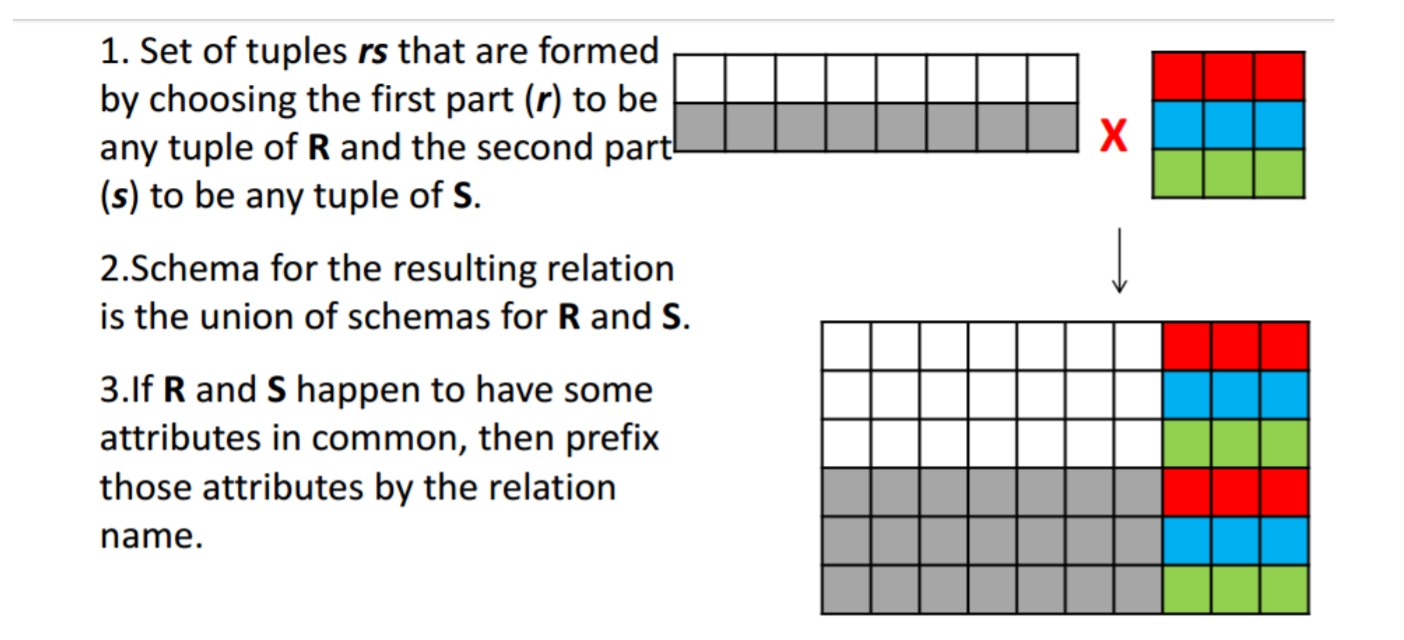
\includegraphics[scale=0.2]{Lec3/cartian.png}

    \item Join: $A\bowtie B$:
    \\is combination of Cartesian product with conditional select.There are many type of Joins.\begin{enumerate}
        \item ThetaJoin:$A\bowtie _{Condition}B$\\
        result: $\sigma _{Condition} (A\times B)$
        \item EquiJoin:$A\bowtie _{A.a=B.b}B$\\
        is sub join of ThetaJoin that condition is equility.
        \item NatureJoin:$A\bowtie B$\\
        is sub join of EquiJoin, it will automatically compare all the attributes in both tables. must use dot notation.
        \begin{itemize}
            \item Commutative: $R \bowtie S = S \bowtie R$ \\
            attribute order may vary
            \item Associative: $R \bowtie (S \bowtie T) = (R \bowtie S) \bowtie T$
            \item So when writing n-ary joins, brackets are irrelevant.\\ $R1 \bowtie R2 \bowtie . . . \bowtie Rn $
        \end{itemize}
    \end{enumerate}
    \item Assignment: $ R = Expression$ or $R{(A1, ..., An) }=Expression$\\
    result:You get a new relation named R It allow you rename attributes. \\R must be a temporary variable, which means you are not changing name in original schema.
    \item Renaming Operator $\rho _{S(A1,A2,A3...An)}(R)$\\
    result: Original R but named S, and all attributes in S are renamed in (A1,A2,A3...An).\\
    when rename part of attributes, use $\rho _{S,A1\rightarrow A2,A3\rightarrow A4}(R)$
    \item Set operations:\begin{enumerate}
        \item $A\cup B$,$A\cap B$: \\Tuples in A or B, Tuples in A and B.
        \item $A-B$: \\Tuples in A that not in B. \\*$A-B\ne B-A$
    \end{enumerate}
    \item dangling :\\
        When we try to nature join two tables:$A\bowtie B$,We will lose all the tuple that mismatch each others. those tuple are called dangling tuple.
    \item Outer Join: \\
    A sub join of Nature Join, that will keep dangliang tuple and filling the missing information by Null.
    \begin{enumerate}
        \item Left Outer Join:$A\ltimes _{Condition} B$:\\Only keep the dangling from left side.
        \item Right Outer Join:$A\rtimes _{Condition} B$:\\Only keep the dangling from right side.
        \item Full Outer Join: $A\times _{Condition}B$:\\Keep dangling in both sides.
    \end{enumerate} 
        

\end{enumerate}